\chapter{Основы}
\label{chap:basics}

\epigraph{Трейси: Я не знал, что ты была там.\\
Зоуи: В каком-то смысле. Невидимость — ты, вероятно, слышал о ней.\\
Трейси: Не думаю, что это было в базовом курсе.
}{Из 14-го эпизода <<Firefly>>, <<Сообщение>>.}



\section{Некоторые базовые понятия в вычислениях}

\section{Асимптотическая нотация}
\subsection{Это какая-то китайская грамота!}
\subsection{Основные термины и правила}
\subsection{Рассмотрим асимптотики поближе}
\subsection{Three Important Cases}
\subsection{Эмпирическая оценка алгоритмов}
\label{sec:empirical-evaluation}

В этой книге описывается\textit{ проектирование алгоритмов} (и тесно связанный с ним\textit{ анализ алгоритмов}). Но в разработке есть также и другой немаловажный процесс, жизненно необходимый при создании крупных реальных проектов, это — \textit{оптимизация алгоритмов}, искусство их \textit{эффективной реализации}. С точки зрения такого разделения, проектирование алгоритма можно рассматривать как способ достижения низкой асимптотической сложности алгоритма (с помощью разработки эффективного алгоритма), а оптимизацию — как уменьшение констант, скрытых в этой асимптотике.

Хотя я могу дать несколько советов по алгоритмам проектирования в Python, сложно угадать, какие именно хитрости и уловки дадут вам лучшую производительность в конкретной задаче, над которой вы работаете, или для вашего оборудования и версии Python. (Асимптотики используются как раз для того, чтобы не было нужды прибегать к таким вещам). Вообще, в некоторых случаях хитрости могут вовсе не потребоваться, потому что ваша программа и так достаточно быстра. Самое простое, что вы можете сделать в большинстве случаев, это просто пробовать и смотреть. Если у вас \textit{есть идея} какого-то хака, то просто опробуйте ее! Реализуйте свою хитрость и запустите несколько тестов. Есть ли улучшения? А если это изменение делает ваш код менее читаемым, а прирост производительности мал, то подумайте — стоит ли оно того?

\begin{note}
Этот раздел рассказывает об оценке алгоритмов, а не об их оптимизации. В приложении \ref{app:A} есть несколько советов по ускорению программ на Python.
\end{note}

Есть ряд теоретических аспектов так называемой экспериментальной алгоритмики (то есть, экспериментальной оценки алгоритмов и их реализации), но они выходят за рамки этой книги, так что я дам вам несколько практических советов, которые могут быть весьма полезны.

\subsubsection*{Совет 1. Если возможно, то не беспокойтесь об этом}

Беспокойство об асимптотической сложности может быть очень полезным. Иногда \textit{решение} задачи из-за сложности на практике может \textit{перестать} быть таковым. Однако, постоянные константы в асимптотике часто совсем не критичны. Попробуйте простую реализацию алгоритма для начала, и убедитесь, что она работает стабильно. (В принципе, вы можете сначала попробовать примитивный алгоритм. Гуру программирования Кен Томпсон писал: «Когда вы в затруднении, используйте перебор вариантов». Перебор вариантов в алгоритмах обычно означает попытку попробовать каждое из возможных решений, при этом временные затраты будут безумными!) Если все работает — оставьте как есть.

\subsubsection*{Совет 2. Для измерения времени работы используйте \texttt{timeit}}

Модуль \texttt{timeit} предназначен для измерения времени работы. Хотя для получения действительно надежных данных вам потребуется выполнить кучу работы, для практических целей timeit вполне сгодится. Например:

\begin{lstlisting}
>>> import timeit
>>> timeit.timeit("x = 2 + 2")
0.034976959228515625
>>> timeit.timeit("x = sum(range(10))")
0.92387008666992188
\end{lstlisting}

Модуль timeit можно использовать прямо из командной строки, например:

\begin{lstlisting}
python -m timeit -s"import mymodule as m" "m.myfunction()"
\end{lstlisting}

Существует кое-что, с чем вы должны быть осторожны при использовании \texttt{timeit}: побочные эффекты, которые будут влиять на повторное исполнение \texttt{timeit}. Функция \texttt{timeit} будет запускать ваш код несколько раз, чтобы увеличить точность, и если прошлые запуски влияют на последующие, то вы окажетесь в затруднительном положении. Например, если вы измеряете скорость выполнения чего-то вроде \texttt{mylist.sort()}, список будет отсортирован только \textit{в первый раз}. Во время остальных тысяч запусков список уже будет отсортированным и это даст нереально маленький результат.

Больше информации об этом модуле и о том, как он работает, можно найти в документации стандартной библиотеки Python.

\subsubsection*{Совет 3. Чтобы найти узкие места, используйте профайлер}

Часто, для того чтобы понять, какие части программы требуют оптимизации, делаются разные догадки и предположения. Такие предположения нередко оказываются ошибочными. Вместо того, чтобы гадать, воспользуйтесь профайлером. В стандартной поставке Python идет несколько профайлеров, но рекомендуется использовать \texttt{cProfile}. Им так же легко пользоваться, как \texttt{timeit}, но он дает больше подробной информации о том, на что тратится время при выполнении программы. Если основная функция вашей программы называется \texttt{main}, вы можете использовать профайлер следующим образом:

\begin{lstlisting}
import cProfile
cProfile.run('main()')
\end{lstlisting}

Такой код выведет отчет о времени работы различных функций программы. Если в вашей системе нет модуля \texttt{cProfile}, используйте \texttt{profile} вместо него. Больше информации об этих модулях можно найти в документации. Если же вам не так интересны детали \textit{реализации}, а просто нужно оценить поведение \textit{алгоритма} на конкретном наборе данных, воспользуйтесь модулем \texttt{trace} из стандартной библиотеки. С его помощью можно посчитать, сколько раз будут выполнены то или иное выражение или вызов в программе.

\subsubsection*{Совет 4. Показывайте результаты графически}

Визуализация может стать прекрасным способом, чтобы понять что к чему. Для исследования производительности часто применяются \textit{графики} (например, для оценки связи количества данных и времени исполнения) и диаграммы типа \textit{<<ящик с усами>>}, отображающие распределение временных затрат при нескольких запусках. Примеры можно увидеть на рисунке \ref{fig:evaluation-diagrams}.

\begin{figure}[h]
	\centering
	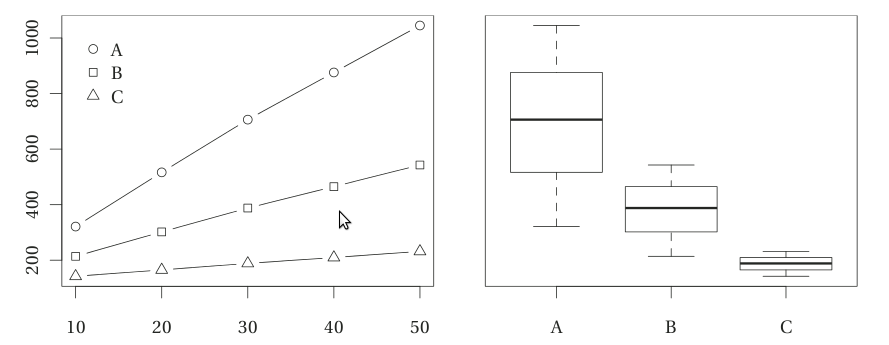
\includegraphics[width=\textwidth]{img/2-2.png}
	\caption{Визуализация времени работы для программ A, B и C и размеров данных 10 "--- 50}
	\label{fig:evaluation-diagrams}
\end{figure}

Отличная библиотека для построения графиков и диаграмм из Python "--- matplotlib (можно взять на \url{http://matplotlib.sf.net}).

\subsubsection*{Совет 5. Будьте внимательны в выводах, основанных на сравнении времени работы}

Этот совет довольно расплывчатый, потому что существует много ловушек, в которые можно попасть, делая выводы о том, какой способ лучше, на основании сравнения времени работы. Во-первых, любая разница, которую вы видите, может определяться случайностью. Если вы используете специальные инструменты вроде \texttt{timeit}, риск такой ситуации меньше, потому что они повторяют измерение времени вычисления выражения несколько раз (или даже повторяют весь замер несколько раз, выбирая лучший результат). Таким образом, всегда будут случайные погрешности и если разница между двумя реализациями не превышает некоторой погрешности, нельзя сказать, что эти реализации различаются (хотя и то, что они одинаковы, тоже \textit{нельзя} утверждать).

\begin{note}
Если вам нужно сделать выводы быстро, можно воспользоваться методом проверки статистических гипотез. Однако, на практике, если различия действительно очень малы, то, вероятно, неважно, какую реализацию вы выберете, так что используйте ту, что больше нравится.
\end{note}

Проблема усложняется, если вы сравниваете больше двух реализаций. Количество пар для сравнения увеличивается пропорционально \textit{квадрату} количества сравниваемых версий, \textit{сильно} увеличивая вероятность того, что как минимум две из версий будут казаться слегка различными. (Это называется проблемой \textit{множественного сравнения}). Существуют статистические решения этой проблемы, но самый простой способ "--- повторить эксперимент с двумя подозрительными версиями. Возможно, потребуется сделать это несколько раз. Они по-прежнему выглядят похожими?

Во-вторых, есть несколько моментов, на которые нужно обращать внимание при сравнении средних величин. Как минимум, вы должны сравнивать средние значения реального времени работы. Обычно, чтобы получить показательные числа при измерении производительности, время работы каждой программы нормируется делением на время выполнения какого-нибудь стандартного, простого алгоритма. Действительно, это может быть полезным, но в ряде случаев сделает бессмысленными результаты замеров. Несколько полезных указаний на эту тему можно найти в статье <<How not to lie with statistics: The correct way to summarize benchmark results>> Fleming и Wallace. Также можно почитать Bast и Weber <<Don't compare averages>>, или более новую статью Citron и др. <<The harmonic or geometric mean: does it really matter?>>

И в-третьих, возможно, ваши выводы нельзя обобщать. Подобные измерения на другом наборе входных данных и на другом железе могут дать другие результаты. Если кто-то будет пользоваться результатами ваших измерений, \textit{необходимо последовательно задокументировать}, каким образом вы их получили.

\subsubsection*{Совет 6. Будьте осторожны, делая выводы об асимптотике из экспериментов}

Если вы хотите что-то сказать окончательно об асимптотике алгоритма, то необходимо проанализировать ее, как описано ранее в этой главе. Эксперименты могут дать вам намеки, но они очевидно проводятся на конечных наборах данных, а асимптотика "--- это то, что происходит при сколь угодно больших размерах данных. С другой стороны, если только вы не работаете в академической сфере, \textit{цель} асимптотического анализа "--- сделать какой-то вывод о поведении алгоритма, реализованного конкретным способом и запущенного на определенном наборе данных, а это значит, что измерения \textit{должны быть} соответствующими.

Например, вы \textit{предполагаете}, что алгоритм работает с квадратичной сложностью, но вы не можете окончательно доказать это. Можете ли вы использовать эксперименты для доказательства вашего предположения? Как уже говорилось, эксперименты (и оптимизация алгоритмов) имеют дело в основном с постоянными коэффициентами, но \textit{выход есть}. Основной проблемой является то, что ваша гипотеза на самом деле непроверяема экспериментально. Если вы утверждаете, что алгоритм имеет сложность $O(n^2)$, то данные не могут это ни подтвердить, ни опровергнуть. Тем не менее, если вы сделаете вашу гипотезу более \textit{конкретной}, то она станет проверяемой. Вы могли бы, например, основываясь на некоторых данных положить, что время работы программы никогда не будет превышать $0.24n^2+0.1n+0.03$ секунд в вашем окружении. Это проверяемая (точнее, \textit{опровергаемая}) гипотеза. Если вы сделали множество измерений, но так и не можете найти контр-примеры, значит ваша гипотеза может быть верна. А это уже и подтверждает гипотезу о квадратичной сложности алгоритма.

\section{Реализация графов и деревьев }
\label{sec:implementing-graphs-and-trees}
Первая задача из главы \ref{chap:intro}, в которой нам требовалось объехать Швецию и Китай, была примером задачи, которая может быть решена с помощью одного из мощнейших инструментов "--- с помощью \textit{графов}. Часто, если вы можете определить, что решаете задачу на графы, вы по-крайней мере на полпути к решению. А если ваши данные можно каким-либо образом представить как \textit{деревья}, у вас есть все шансы построить действительно \textit{эффективное} решение.

Графами можно представить любую структуру или систему, от транспортной сети до сети передачи данных и от взаимодействия белков в ядре клетке до связей между людьми в Интернете.
Ваши графы могут стать еще полезнее, если вы добавите в них дополнительные данные вроде \textit{весов} или \textit{расстояний}, что даст возможность описывать такие разнообразные проблемы как игру в шахматы или определение подходящей работы для человека в соответствии с его способностями.
Деревья — это просто особый вид графов, так что большинство алгоритмов и представлений графов сработают и для них.
Однако, из-за их особых свойств (связанность и отсутствие циклов), можно применить специальные (и весьма простые) версии алгоритмов и представлений.
На практике в некоторых случаях встречаются структуры (такие как XML-документы или иерархия каталогов), которые могут быть представлены в виде деревьев\footnote{С учетом атрибутов IDREF и символьных ссылок XML-документы и иерархия каталогов становятся собственно графами.}. На самом деле эти <<некоторые>> случаи довольно-таки общие.

Если вы забыли терминологию (или ее и не знали), почитайте приложение \ref{app:graph-theory}, <<Терминология теории графов>>. Здесь же опишем основные моменты:

\begin{itemize}
\item Граф $G = (V, E)$ состоит из \textit{вершин}, $V$, и \textit{ребер} между ними, $E$. Если ребра имеют направление, то граф называется \textit{направленным}.
\item Вершины, связанные ребром, называются \textit{смежными}. Соединяющее две вершины ребро называется \textit{инцидентным} с ними. Вершины, смежные с $v$ называются \textit{соседними} с $v$.
\item \textit{Подграф} графа $G = (V,E)$ состоит из подмножества $V$ и подмножества $E$. \textit{Путь} в графе "--- это подграф, вершины которого соединены ребрами последовательно, причем каждая вершина включена только один раз. \textit{Цикл} — это то же самое, что и путь, только последнее его ребро связывает последнюю вершину с первой.
\item Если каждому ребру в $G$ будет сопоставлено определенное значение (\textit{вес}), то $G$ будет называться \textit{взвешенным} графом. \textit{Длина} пути или цикла — это сумма всех весов его ребер или, для невзвешенных графов, просто количество ребер.
\item \textit{Лесом} называется граф без циклов, а связанный граф — это \textit{дерево}. Иными словами, лес состоит из одного или многих деревьев.
\end{itemize}

Описание задачи в терминах графов является довольно абстрактным, так что если вам нужно реализовать решение, вы должны представить графы в виде каких-либо структур данных. (Это придется делать даже при проектировании алгоритма и только, потому что нужно знать, сколько времени будут выполняться различные операции на представлении графа). В некоторых случаях граф будет уже составлен в коде или данных, так что отдельной структуры не потребуется. Например, если вы пишете веб-краулер, собирающий информацию о сайтах по ссылкам, графом будет сама сеть. Если у вас есть класс \texttt{Person} с атрибутом \texttt{friends}, являющимся списком других объектов типа \texttt{Person}, то ваша объектная модель уже будет графом, на котором можно использовать различные алгоритмы. Однако существуют и специальные способы представления графов.

В общих словах, мы ищем способ реализации функции смежности, $N(v)$, так, чтобы \texttt{N[v]} было каким-либо набором (или в отдельных случаях просто итератором) смежных с \texttt{v} вершин. Как и во многих других других книгах мы сосредоточимся на двух наиболее известных представлениях: \textit{списках смежности} и \textit{матрицах смежности}, потому что они наиболее полезны и обобщены. Альтернативные представления описаны в разделе \ref{sec:multitude-representation} ниже.

\begin{notice}{Словари и множества}

Существует техника, подробно описываемая в большинстве книг об алгоритмах, и обычно очевидная для программистов на Python, это "--- \textit{хэширование}. Хэширование подразумевает вычисление целого числа (часто выглядящего как случайное), основанного на произвольном объекте. Потом это значение можно будет использовать, например, как индекс в массиве (после некоторых преобразований, чтобы не выйти за границы массива).

Стандартный механизм хэширования в Python представлен функцией \texttt{hash}:
\begin{lstlisting}
>>> hash(42)
42
>>> hash("Hello, world!")
-1886531940
\end{lstlisting}

Этот механизм используется в словарях, реализованных как так называемые \textit{хэш-таблицы}. Множества реализованы тем же способом. Важная особенность в том, что хэш может быть вычислен по существу за константное время (оно постоянно относительно размера хэш-таблицы, но линейно зависит от размера хэшируемого объекта). Если существует достаточно большой массив, то доступ к нему с помощью хэша в среднем занимает $\Theta(1)$. (В худшем случае это займет $\Theta(n)$, если только мы не знаем значений заранее и не напишем собственную хэш-функцию. Но в любом случае, на практике хэширование очень эффективно). 

Для нас это значит, что доступ к элементам в \texttt{dict} или \texttt{set} происходит за постоянное время, а это делает делает их в высшей степени полезными строительными блоками для более сложных структур и алгоритмов.
\end{notice}


\subsection{Списки смежности и тому подобное}
\label{sec:adjacency-lists}

Один из наиболее очевидных способов представления графов "--- это списки смежности. Смысл их в том, что для каждой вершины создается список (или множество, или другой контейнер или итератор) смежных с ней вершин. Разберем простейший способ реализации такого списка, предположив, что имеется $n$ вершин, пронумерованных $0\ldots n-1$.

\begin{note}
Само собой, вершины могут быть представлены любыми объектами и иметь собственные метки или имена. Однако использование целых чисел в диапазоне $0\ldots n-1$ делает реализацию многих представлений проще, потому что в таком случае номера вершин можно использовать как индексы.
\end{note}

Таким образом, каждый список смежности является списком таких номеров, а сами списки собрать в главный список размера $n$, индексированный номерами вершин. Обычно сортировка таких списков случайная, так что речь в действительности идет об использовании списков для реализации \textit{множеств} смежности. Термин \textit{список} просто исторически устоялся. Python, к счастью, имеет отдельный тип для множеств, который во многих случаев удобно использовать.

Примерный граф, для которого будут показаны разные представления, изображен на рис. \ref{fig:sample-graph}. Для начала положим, что все вершины пронумерованы ($a=0, b =1, \ldots$). С учетом этого граф можно представить очевидным способом, как показано в листинге \ref{lst:main-graph}. Чтобы было удобнее, я присвоил номера вершин переменным, названным в соответствии с метками вершин на рисунке. Но можно работать и прямо с числами. Какой вершине какой список принадлежит указано в комментариях. Если хотите, потратьте несколько минут, чтобы убедиться, что представление соответствует рисунку.

\begin{lstlisting}[caption={Простая реализация представления в виде множеств смежности}, label={lst:main-graph}]
a, b, c, d, e, f, g, h = range(8)

N = [
		{b, c, d, e, f}, # a
		{c, e}, # b
		{d}, # c
		{e}, # d
		{f}, # e
		{c, g, h}, # f
		{f, h}, # g
		{f, g} # h
]
\end{lstlisting}

\begin{note}
В версиях Python до 2.7 (или 3.0) нужно описывать множества как \texttt{set([1, 2, 3])} вместо \texttt{\{1, 2, 3\}}. Но пустое множество в новых версиях по-прежнему записывается как \texttt{set()}, потому что \texttt{\{\}} объявляет пустой словарь.
\end{note}


\tikzstyle{tree} = [circle,
						fill=white!90!black!10,
						drop shadow]

\begin{figure}[h]
\centering
\begin{tikzpicture}
[level/.style={sibling distance=35mm/#1},style={>=latex,->}]
    \tikzstyle{every node}=[circle,draw,text centered,minimum height=2.5em]
    \tikzstyle{every path}=[-latex,draw]

    \node[tree] (a) {\Large $a$};
    \node[tree] (b) [above right=of a] {\Large $b$};
    \node[tree] (c) [right=1.5cm of b] {\Large $c$};
    \node[tree] (d) [below right=of a] {\Large $d$};
    \node[tree] (e) [right=1.5cm of d] {\Large $e$};
    \node[tree] (f) [above right=of e,below right=of c] {\Large $f$};
    \node[tree] (g) [right=3cm of c] {\Large $g$};
    \node[tree] (h) [right=3cm of e] {\Large $h$};

	\path (a) -- (b);
	\path (a) -- (d);
	\path (a) -- (c);
	\path (a) -- (f);
	\path (a) -- (e);
	\path (b) -- (c);
	\path (b) -- (e);
	\path (c) -- (d);
	\path (d) -- (e);
	\path (e) -- (f);
	\path (f) -- (c);
	
	\path (f) edge[bend left=10] (g);
	\path (g) edge[bend left=10] (f);

	\path (h) edge[bend left=10] (g);
	\path (g) edge[bend left=10] (h);

	\path (f) edge[bend left=10] (h);
	\path (h) edge[bend left=10] (f);
\end{tikzpicture}

\caption{Примерный граф для демонстрации разных видов представления}
\label{fig:sample-graph}
\end{figure}

Имя \texttt{N} из листинга связано с функцией $N$, описанной выше. В теории графов $N(v)$ представлет множество смежных с $v$ вершин. Так же и в нашем коде \texttt{N[v]} является множеством смежных с \texttt{v} вершин. Предполагая, что \texttt{N} определена как в примере выше, в интерактивном режиме Python можно поизучать это представление:
\begin{lstlisting}
>>> b in N[a]
True # смежная?
>>> len(N[f])
3 # степень
\end{lstlisting}


\begin{note}[Совет:]
Если у вас есть определенный код в файле, например, определение графа из листинга \ref{lst:main-graph}, и вы хотите запустить этот код в интерактивном режиме, как в предыдущем примере, вам нужно запустить \texttt{python} с ключом \texttt{-i}, например так:

\texttt{python -i listing\_2\_1.py}

Эта команда запустит код из файла и откроет интерактивный интерпретатор, который продолжит работать в том месте, где закончился код в файле, сохранив таким образом все сделанные раньше объявления.
\end{note}

Другим возможным представлением, которое в некоторых случаях даст меньше накладных расходы, являются собственно \textit{списки} смежности. Пример такого списка приведен в листинге \ref{lst:adj-list}. Доступны все те же операции, но проверка смежности вершины выполняется за $\Theta(n)$. Это дает серьезное снижение скорости, но если вам действительно требуется это представление, то это его единственная проблема. (Если все, что делает ваш алгоритм "--- это обход соседних вершин, то использование объектов типа множество не только просто бессмысленно: накладные расходы могут ухудшить постоянные множители в асимптотике вашей реализации).

\begin{lstlisting}[caption={Списки смежности}, label={lst:adj-list}]
a, b, c, d, e, f, g, h = range(8)
N = [
		[b, c, d, e, f], # a
		[c, e], # b
		[d], # c
		[e], # d
		[f], # e
		[c, g, h], # f
		[f, h], # g
		[f, g] # h
]
\end{lstlisting}

Можно поспорить, что это представление на самом деле "--- набор \textit{массивов смежности}, а не классические \textit{списки} смежности, т.к. тип список в Python в действительности является динамическим массивом (см. выше врезку о списках). Если хотите, вы можете реализовать тип связанного списка и использовать его вместо типа \texttt{list} из Python. Это может сделать дешевле в плане производительности произвольные вставки в список, но вам, вероятно, и не понадобится такая операция, потому что с тем же успехом можно добавлять новые вершины к концу списка. Преимущество использования встроенного \texttt{list} в том, что он представляет собой очень быструю и хорошо отлаженную структуру (в отличие от любых структур списков, которые можно реализовать на чистом Python).

При работе с графами постоянно всплывает идея о том, что лучшее представление зависит от того, что именно нужно сделать с графом. Например, используя списки (или массивы) смежности можно сохранить накладные расходы небольшими и обеспечить эффективный обход $N(v)$ для любой вершины $v$. Однако, проверка, являются ли $u$ и $v$ смежными, потребует времени $\Theta(N(v))$, что может стать проблемой при высокой плотности графа (т.е. при большом числе ребер). В этих случаях на помощь придут множества смежности. 

\begin{note}[Совет:]
Было показано, что удаление объектов из середины \texttt{list} в Python довольно затратно. Удаление с \textit{конца} при этом происходит за константное время. Если вы не заботитесь о порядке вершин, то можете удалять случайную вершину за константное время перезаписывая ее той, что находится в конце списка смежности, и вызывая затем метод \texttt{pop}.
\end{note}

Небольшой вариацией на тему этого представления можно назвать сортированные списки смежных вершин. Если списки нечасто меняются, их можно держать отсортированными и использовать бисекцию (см. врезку о бисекции в главе \ref{chap:divide-combine}) для проверки смежности вершины, что приведет к немного меньшим накладным расходам (в плане использования памяти и времени итерации), но увеличит сложность проверки до $\Theta(\lg k)$, где $k$ "--- количество смежных с данной вершин. (Это все равно очень маленькое значение. На практике, впрочем, использование встроенного типа \texttt{set} доставляет гораздо меньше хлопот).

\textit{Еще одна} небольшая доработка заключается в использовании словарей вместо множеств или списков. Смежные вершины могут быть ключам словаря, а в качестве значения можно использовать любые дополнительные данные, например, вес ребра. Как это выглядит можно увидеть в листинге \ref{lst:weighted-dict} (веса выбраны случайно).

\begin{lstlisting}[caption={Словарь смежности с весами ребер}, label={lst:weighted-dict}]
a, b, c, d, e, f, g, h = range(8)
N = [
		{b:2, c:1, d:3, e:9, f:4}, # a
		{c:4, e:3}, # b
		{d:8}, # c
		{e:7}, # d
		{f:5}, # e
		{c:2, g:2, h:2}, # f
		{f:1, h:6}, # g
		{f:9, g:8} # h
]
\end{lstlisting}

Словарь смежности можно использовать точно так же как и другие представления, с учетом дополнительной информации о весах:
\begin{lstlisting}
>>> b in N[a]	# смежность
True
>>> len(N[f])	# степень
3
>>> N[a][b]		# вес (a, b)
2
\end{lstlisting}

Если хотите, можете использовать словари смежности даже если у вас \textit{нет} полезных данных вроде весов ребер (используя \texttt{None} или другое значение для замещения данных). Это даст вам все преимущества множеств смежности, но при этом будет работать с (очень-очень) старыми версиями Python, не имеющими поддержки типа \texttt{set}\footnote{Множества были введены в Python 2.3 в виде модуля \texttt{sets}. Встроенный тип \texttt{set} доступен начиная с Python 2.4.}.

До этого момента структура, хранящая структуры смежности "--- списки, множества или словари "--- была списком, индексированным номерами вершин. Более гибкий вариант (позволяющий использовать произвольные, хэшируемые, имена вершин) строится на базе словаря в качестве основной структуры\footnote{Такие словари со списками смежности Гвидо ван Россум использовал в своей статье <<Python Patterns "--- Implementing Graphs>>, выложенной по адресу \url{http://www.python.org/doc/essays/graphs.html}.}. Листинг \ref{lst:dict-based} показывает пример словаря, содержащего множества смежности. Заметьте, что вершины в нем обозначены символами.

\begin{lstlisting}[caption={Словарь с множествами смежности}, label={lst:dict-based}]
N = {
		'a': set('bcdef'),
		'b': set('ce'),
		'c': set('d'),
		'd': set('e'),
		'e': set('f'),
		'f': set('cgh'),
		'g': set('fh'),
		'h': set('fg')
}
\end{lstlisting}

\begin{note}
Если из листинга \ref{lst:dict-based} выбросить конструктор \texttt{set}, то останутся \textit{строки} смежности, которые будут работать как списки смежности (неизменяемые) из символов (с чуть меньшими накладными расходами). Казалось бы, далеко не лучшее представление, но, как и было сказано выше, все зависит от вашей программы. Откуда вы получаете данные для графа? (Может быть, они уже в виде текста?) Как вы собираетесь их использовать?
\end{note}

\subsection{Матрицы смежности}
\label{sec:adjacency-matrix}

Другая распространенная форма представления графов — это матрицы смежности. Основное отличие их в следующем: вместо перечисления всех смежных с каждой из вершин, мы записываем один ряд значений (массив), каждое из которых соответствует возможной смежной вершине (есть хотя бы одна такая для каждой вершины графа), и сохраняем значение (в виде \texttt{True} или \texttt{False}), показывающее, действительно ли вершина является смежной. И вновь простейшую реализацию можно получить используя вложенные списки, как видно из листинга \ref{lst:adjacency}. Заметьте, что это также требует, чтобы вершины были пронумерованы от $0$ до $V-1$. В качестве значений истинности используются 1 и 0 (вместо \texttt{True} и \texttt{False}), чтобы сделать матрицу читабельной.

\begin{lstlisting}[caption={Матрица смежности, реализованная с помощью вложенных списков},label={lst:adjacency}]
a, b, c, d, e, f, g, h = range(8)
	    # a b c d e f g h

N = [[0,1,1,1,1,1,0,0], # a
		 [0,0,1,0,1,0,0,0], # b
		 [0,0,0,1,0,0,0,0], # c
		 [0,0,0,0,1,0,0,0], # d
		 [0,0,0,0,0,1,0,0], # e
		 [0,0,1,0,0,0,1,1], # f
		 [0,0,0,0,0,1,0,1], # g
		 [0,0,0,0,0,1,1,0]] # h
\end{lstlisting}

Способ использования матриц смежности слегка отличается от списков и множеств смежности. Вместо проверки входит ли $b$ в $N[a]$, вы будете проверять, истинно ли значение ячейки матрицы $N[a][b]$. Кроме того, больше нельзя использовать $len(N[a])$, чтобы получить количество смежных вершин, потому что все ряды одной и той же длины. Вместо этого можно использовать функцию \texttt{sum}:
\begin{lstlisting}
>>> N[a][b]
1
>>> sum(N[f])
3
\end{lstlisting}

Матрицы смежности имеют ряд полезных свойств, о которых стоит знать. Во-первых, так как мы не рассматриваем графы с петлями (т.е. не работаем с псевдографами), все значения на диагонали — ложны. Также, ненаправленные графы обычно описываются парами ребер в обоих направлениях. Это значит, что матрица смежности для ненаправленного графа будет симметричной.

Расширение матрицы смежности для использования весов тривиально: вместо сохранения логических значений, сохраняйте значения весов. В случае с ребром $(u, v)$ $N[u][v]$ будет весом ребра $w(u,v)$ вместо \texttt{True}. Часто в практических целях несуществующим ребрам присваиваются бесконечные веса. (Это гарантирует, что они не будут включены, например, в кратчайшие пути, т. к. мы ищем путь по существующим ребрам). Не всегда очевидно, как представить бесконечность, но совершенно точно есть несколько разных вариантов.

Один из них состоит в том, чтобы использовать некорректное для веса значение, такое как \texttt{None} или $-1$, если известно, что все веса неотрицательны. Возможно, в ряде случаев полезно использовать действительно большие числа. Для целых весов можно применить \texttt{sys.maxint}, хотя это значение и не обязательно самое большое (длинные целые могут быть больше). Есть и значение, введенное для отражения бесконечности: \texttt{inf}. Оно недоступно в Python напрямую по имени и выражается как \texttt{float('inf')}\footnote{Гарантируется, что это работает для Python 2.6 и старше. В ранних версиях подобные специальные значения были платформо-зависимы, хотя \texttt{float('inf')} или \texttt{float('Inf')} должны сработать на большинстве платформ.}.

Листинг \ref{lst:adjacency-weighted} показывает, как выглядит матрица весов, реализованная вложенными списками. Использованы те же веса, что и в листинге \ref{lst:adjlist-weighted}.

\begin{lstlisting}[caption={Матрица весов с бесконечными значениями для отсутствующих ребер}, label={lst:adjacency-weighted}]
a, b, c, d, e, f, g, h = range(8)
_ = float('inf')

		# a b c d e f g h

W = [[0,2,1,3,9,4,_,_], # a
	 	 [_,0,4,_,3,_,_,_], # b
		 [_,_,0,8,_,_,_,_], # c
		 [_,_,_,0,7,_,_,_], # d
		 [_,_,_,_,0,5,_,_], # e
		 [_,_,2,_,_,0,2,2], # f
		 [_,_,_,_,_,1,0,6], # g
		 [_,_,_,_,_,9,8,0]] # h
\end{lstlisting}

Бесконечное значение обозначено как подчеркивание (\texttt{\_}), потому что это коротко и визуально различимо. Естественно, можно использовать любое имя, которое вы предпочтете. Обратите внимание, что значения на диагонали по-прежнему равны нулю, потому что даже без учета петель, веса часто интерпретируются как расстояния, а расстояние от вершины до самой себя равно нулю.

Конечно, матрицы весов дают возможность очень просто получить веса ребер, но, к примеру, проверка смежности и определение степени вершины, или обход всех смежных вершин делаются иначе. Здесь нужно использовать бесконечное значение, примерно так (для большей наглядности определим \texttt{inf = float('inf')}):
\begin{lstlisting}
>>> W[a][b] < inf # смежность
True
>>> W[c][e] < inf # смежность
False
>>> sum(1 for w in W[a] if w < inf) - 1 # степень
5
\end{lstlisting}

Заметьте, что из полученной степени вычитается $1$, потому что мы не считаем значения на диагонали. Сложность вычисления степени тут $\Theta(n)$, в то время как в другом представлении и смежность, и степень вершины можно определить за константное время. Так что  вы всегда должны понимать, \textit{как именно} вы собираетесь использовать ваш граф и выбирать для него соответствующее представление.

\begin{notice}{Массивы специального назначения из NumPy}

Библиотека NumPy содержит много функциональности, связанной с многомерными массивами. Для представления графов большая ее часть не нужна, но массивы из NumPy весьма полезны, например, для реализации матриц весов или смежности.

Вместо создания пустой матрицы весов или смежности из списков для $n$ вершин, вроде такого:
\begin{lstlisting}
>>> N = [[0]*10 for i in range(10)]
\end{lstlisting}
в NumPy можно использовать функцию \texttt{zeros}:
\begin{lstlisting}
>>> import numpy as np
>>> N = np.zeros([10,10])
\end{lstlisting}

Отдельные элементы доступны по индексам, разделенным запятой: $A[u,v]$. Чтобы получить соседние с данной вершины, используется одиночный индекс: $A[u]$.

Пакет NumPy можно получить по адресу \url{http://numpy.scipy.org}.

Имейте ввиду, что вам нужна та версия NumPy, что будет работать с вашей версией Python. Если последний релиз NumPy не поддерживает ту версию Python, что вы используете, вы можете скомпилировать и установить библиотеку прямо из репозитория исходных кодов. Исходный код можно получить с помощью следующих команд (предполагается, что у вас установлена Subversion):

\texttt{svn co http://svn.scipy.org/svn/numpy/trunk numpy}

Больше информации о том, как компилировать и устанавливать NumPy, так же как и подробную документацию, можно найти на сайте библиотеки.

\end{notice}

\subsection{Реализация деревьев}

Любое представление графов, естественно, можно использовать для представления деревьев, потому что деревья "--- это особый вид графов. Однако, деревья играют свою большую роль в алгоритмах, и для них разработано много соответствующих структур и методов. Большинство алгоритмов на деревьях (например, поиск по деревьям, описанный в главе \ref{chap:divide-combine}) можно рассматривать в терминах теории графов, но специальные структуры данных делают их проще в реализации. 

Проще всего описать представление дерева с корнем, в котором ребра спускаются вниз от корня. Такие деревья часто отображают иерархическое ветвление данных, где корень отображает все объекты (которые, возможно, хранятся в листьях), а каждый внутренний узел показывает объекты, содержащиеся в дереве, корень которого "--- этот узел. Это описание можно использовать, представив каждое поддерево списком, содержащим все его поддеревья-потомки. Рассмотрим простое дерево, показанное на рисунке \ref{fig:simple-tree}.

Мы можем представить это дерево как список списков:
\begin{lstlisting}
>>> T = [["a", "b"], ["c"], ["d", ["e", "f"]]]
>>> T[0][1]
'b'
>>> T[2][1][0]
'e'
\end{lstlisting}

Каждый список в сущности является списком потомков каждого из внутренних узлов. Во втором примере мы обращаемся к третьему потомку корня, затем ко второму его потомку и в конце концов "--- к первому потомку предыдущего узла (этот путь отмечен на рисунке).


\begin{figure}[h]
\centering
\begin{tikzpicture}[level/.style={sibling distance=35mm/#1},style={>=latex,->}]
    \tikzstyle{every node}=[circle,draw,text centered,minimum height=2.5em]
    \node[tree,draw=red] (z) {}
        child { 
			node[tree] {}
			child { node[tree] {\Large $a$} }
			child {	node[tree] {\Large $b$} } 
		}
        child {
            node[tree] {}
			child { node[tree] {\Large $c$} }
        }
        child { 
			node[tree,draw=red] (1) {} 
			child { node[tree] {\Large $d$} }
			child { 
				node[tree,draw=red] (2) {}
				child { node[tree,draw=red] (3) {\Large $e$} }
				child { node[tree] {\Large $f$} }
			}
		}
    ;

	\path[-latex,color=red] (z) edge[bend left=20] (1);
	\path[-latex,color=red] (1) edge[bend left=20] (2);
	\path[-latex,color=red] (2) edge[bend right=20] (3);
\end{tikzpicture}
\caption{Пример дерева с отмеченным путем от корня к листу}
\label{fig:simple-tree}
\end{figure}


В ряде случаев возможно заранее определить максимальное число потомков каждого узла. (Например, каждый узел \textit{бинарного дерева} может иметь до двух потомков). Поэтому можно использовать другие представления, скажем, объекты с отдельным атрибутом для каждого из потомков как в листинге \ref{lst:binary-tree}.

\begin{figure}[h!]
\begin{lstlisting}[caption={Класс бинарного дерева и его использование}, label={lst:binary-tree}]
class Tree:
	def __init__(self, left, right):
		self.left = left
		self.right = right

>>> t = Tree(Tree("a", "b"), Tree("c", "d"))
>>> t.right.left
'c'
\end{lstlisting}
\end{figure}
Для обозначения отсутствующих потомков можно использовать \texttt{None} (в случае если у узла только один потомок). Само собой, можно комбинировать разные методы (например, использовать списки или множества потомков для каждого узла).

Распространенный способ реализации деревьев, особенно на языках, не имеющих встроенной поддержки списков, это так называемое представление <<первый потомок, следующий брат>>. В нем каждый узел имеет два <<указателя>> или атрибута, указывающих на другие узлы, как в бинарном дереве. Однако, первый из этих атрибутов ссылается на первого потомка узла, а второй "--- на его следующего брата\translationnote{т.~е. узел, имеющий того же родителя, но находящийся правее}. Иными словами, каждый узел дерева имеет указатель на связанный список его потомков, а каждый из этих потомков ссылается на свой собственный аналогичный список. Таким образом, небольшая модификация бинарного дерева (листинг \ref{lst:binary-tree}) даст нам многопутевое дерево, показанное в листинге \ref{lst:multiway-tree}.

\begin{figure}[h]
\begin{lstlisting}[caption={Класс многопутевого дерева}, label={lst:multiway-tree}]
class Tree:
	def __init__(self, kids, next=None):
		self.kids = self.val = kids
		self.next = next
\end{lstlisting}
\end{figure}

Отдельный атрибут \texttt{val} здесь введен просто для того, чтобы получить понятный вывод при указании значения (например, <<c>>) вместо ссылки на узел. Естественно, все это можно изменять. Вот пример того, как можно обращаться с этой структурой:
\begin{lstlisting}
>>> t = Tree(Tree("a", Tree("b", Tree("c", Tree("d")))))
>>> t.kids.next.next.val
'c'
\end{lstlisting}

А вот как выглядит это дерево:
\begin{figure}[!h]
\centering
\begin{tikzpicture}[sibling distance=20mm,style={>=latex,->}]
    \tikzstyle{every node}=[circle,draw,text centered,minimum height=2.5em]
    \node[tree] (z) {}
		child { node[tree] (a) {\Large $a$} }
		child {	node[tree] (b) {\Large $b$} } 
		child { node[tree] (c) {\Large $c$} }
		child { node[tree] (d) {\Large $d$} }
    ;
	\draw[-latex,dashed,color=white!20!black!80] (z) .. controls +(west:0.5cm) and +(north east:1.5cm) .. (a) {};
	\draw[-latex,dashed,color=white!20!black!80] (a) -- (b) {};
	\draw[-latex,dashed,color=white!20!black!80] (b) -- (c) {};
	\draw[-latex,dashed,color=white!20!black!80] (c) -- (d) {};
\end{tikzpicture}
\end{figure}

Атрибуты \texttt{kids} и \texttt{next} показаны пунктирными линиями, а сами ребра дерева "--- сплошными. Я немного схитрил и не стал показывать отдельные узлы для строк <<a>>, <<b>> и т.д. Вместо этого я трактую их как метки на соответствующих родительских узлах. В более сложном дереве вместо использования одного атрибута и для хранения значения узла и для ссылки на список потомков, для обеих целей могут понадобиться отдельный атрибуты. Обычно для обхода дерева используется более сложный код (включая циклы и рекурсию), чем приведенный здесь с жестко заданным путем. Больше об этом написано в главе \ref{chap:traversal}. В главе \ref{chap:combine-divide} также обсуждаются многопутевые деревья и балансировка деревьев.

\begin{notice}{Шаблон проектирования <<Набор>>}
При проектировании (да и реализации) таких структур данных как деревья может оказаться полезным гибкий класс, позволяющий задавать набор атрибутов через конструктор. Здесь нас может выручить шаблон проектирования <<Набор>> (названный так Алексом Мартелли в <<Python Cookbook>>). Есть много способов его реализации, но суть видна из следующего кода:
\begin{lstlisting}
class Bunch(dict):
	def __init__(self, *args, **kwds):
		super(Bunch, self).__init__(*args, **kwds)
		self.__dict__ = self
\end{lstlisting}

Есть несколько полезных способов его применения. Во-первых, он позволяет создать и задать значения атрибутов, передав их как аргументы при создании объекта:
\begin{lstlisting}
>>> x = Bunch(name="Jayne Cobb", position="PR")
>>> x.name
'Jayne Cobb'
\end{lstlisting}

Во-вторых, наследование от \texttt{dict} дает много дополнительного функционала, такого как получение всех ключей (атрибутов) или простая проверка наличия атрибута. Вот пример:
\begin{lstlisting}
>>> T = Bunch
>>> t = T(left=T(left="a", right="b"), right=T(left="c"))
>>> t.left
{'right': 'b', 'left': 'a'}
>>> t.left.right
'b'
>>> t['left']['right']
'b'
>>> "left" in t.right
True
>>> "right" in t.right
False
\end{lstlisting}

Конечно же этот шаблон можно использовать не только для создания деревьев. Он пригодится в любой ситуации, где необходим гибкий объект, умеющий задавать свои атрибуты при создании.
\end{notice}

\subsection{Множество разных представлений}
\label{sec:multitude-representation}

Несмотря на то, что существует масса представлений графов, большинство изучают и используют только два вида (с изменениями), уже описанных в этой главе. Джереми Спинред в своей книге <<Effective Graph Representation>> пишет, что его, как исследователя компьютерного представления графов, <<особенно раздражают>> большинство вводных статей. Приводимые в них описания хорошо известных представлений (списков и матриц смежности) обычно адекватны, но более общие объяснения нередко ошибочны. Как пример, он показывает следующий ложный вывод о представлении графов, который основывается на неверных положениях из разных статей:
\textit{<<Существует два метода представления графов в компьютере: списки и матрицы смежности. Работа с матрицами смежности быстрее, но они требуют больше памяти, чем списки смежности, так что вам нужно выбрать один из двух способов, исходя из того, какой ресурс для вас важнее>> (стр. 9).}

Спинред отмечает, что эти заключения сомнительны по нескольким причинам. Во-первых, есть \textit{много} интересных способов представления графов, не только два описанных. Например, существуют \textit{списки ребер} (или \textit{множества ребер}), являющиеся списком всех ребер в виде пар вершин (или специальных объектов-ребер), существуют \textit{матрицы инцидентности}, показывающие, какие ребра каким вершинам инцидентны (полезно для мультиграфов). Также существуют специальные методы для особых типов графов, вроде деревьев (описанных выше) и интервальных графов (здесь не рассматриваются). Полистайте книгу Спинреда, чтобы узнать о представлениях графов, которые вам могут когда-нибудь понадобиться.
Во-вторых, идея компромисса между памятью и временем работы может ввести в заблуждение: есть проблемы, решение которых со списками смежности будет быстрее, чем с матрицами смежности, а для произвольного графа на практике списки смежности требуют \textit{больше} памяти, чем матрицы.

Так что, вместо того, чтобы полагаться на простые обобщенные выводы, подобные описаным, нужно вникнуть в специфику своей задачи. Основным критерием, вероятно, будет асимптотическая сложность того, что вы делаете. Например, поиск ребра $(u, v)$ в матрице смежности выполняется за $\Theta(1)$, а обход смежных с $v$ вершин "--- за $\Theta(n)$, в то время как на списке смежности обе операции будут выполнены за $\Theta(d(v))$, т.е. будут зависеть от количества смежных с данной вершин. 
Если асимптотическая сложность вашего алгоритма не зависит от типа представления, вы можете провести какие-либо эмпирические тесты, описанные ранее в этой главе. Или, как часто и бывает, можно выбрать то представление, которое лучше сочетается с вашим кодом и проще в поддержке.

Важный способ использования графов, который еще не был затронут, не касается их представления. Дело в том, что во многих задачах данные уже имеют структуру графа, или даже дерева, и мы можем использовать для них соответствующие алгоритмы для графов и деревьев без создания специальных представлений. В ряде случаев это происходит, если представление графа составлено вне нашей программы. Например, при разборе XML-документов или обходе каталогов файловой системы древовидная структура уже создана и для нее существуют определенные API. Иными словами, мы \textit{неявно} задаем граф. К примеру, чтобы найти наиболее эффективное решение для заданной конфигурации кубика Рубика, можно определить состояние куба и методы его изменения. Но даже если явно не описывать и не сохранять каждую конфигурацию, \textit{возможные состояния} сформируют неявный граф (или множество вершин) с ребрами "--- операторами изменения состояния. Дальше можно использовать такие алгоритмы, как A* или двунаправленный алгоритм Дейкстры (оба описаны в главе \ref{chap:from-a-to-b}), чтобы найти кратчайший путь до состояния решения. В таких случаях функция получения соседних вершин $N(v)$ будет работать <<на лету>>, вероятно, возвращая смежные вершины как коллекцию или другую форму объекта-итератора.

И последний тип графов, которого я коснусь в этой главе, называется \textit{графом подзадач}. Это глубокая концепция, к которой я еще неоднократно буду обращаться, оисывая различные техники построения алгоритмов. Вкратце, большинство задач может быть разложено на \textit{подзадачи}: меньшие задачи, часто имеющие похожую структуру. Они формируют вершины графа подзадач, а их зависимости (т.е. какая подзадача от какой зависит) выражаются ребрами. И хотя алгоритмы на графы редко применяются на графах подзадач (они используются больше как инструмент анализа), такие графы отлично позволяют понять технику <<разделяй и властвуй>> (глава \ref{chap:combine-divide}) и динамическое программирование (глава \ref{chap:memoiz}).

\begin{notice}{Библиотеки для графов}
Основных методов представления графов, описанных в этой главе, вероятно будет достаточно для большинства ваших задач на графы, особенно при некоторых изменениях. Однако, есть ряд операций, реализация которых может быть неочевидной и запутанной, таких как временной скрытие вершин или их совмещение. Существуют сторонние библиотеки, которые реализуют эти методы и часть из них написана как расширения на C, что при использовании может дать прирост производительности. Они весьма удобны в применении, а в некоторых сразу реализовано несколько алгоритмов на графах. Поиск в интернете даст вам список активно разрабатываемых библиотек для графов, вот несколько для начала:
\begin{itemize*}
\item {\bf NetworkX}: \url{http://networkx.lanl.gov}
\item {\bf python-graph}: \url{http://code.google.com/p/python-graph}
\item {\bf Graphine}: \url{http://gitorious.org/projects/graphine/pages/Home}
\end{itemize*}

Кроме того, существуют Pygr, база данных графов (\url{http://bioinfo.mbi.ucla.edu/pygr}), Gato, набор инструментов для анимации графов (\url{http://gato.sourceforge.net}) и PADS, коллекция алгоритмов на графах (\url{http://www.ics.uci.edu/~eppstein/PADS}).
\end{notice}

\newpage
\section{Beware of Black Boxes}
\subsection{Hidden Squares}
\subsection{The Trouble with Floats}
\section{Заключение}
\section{Если вы заинтересовались…}
\section{Упражнения}
\section{Ссылки}





%%% Local Variables: 
%%% mode: latex
%%% TeX-master: "mapl"
%%% End: 
